\documentclass[conference]{IEEEtran}
\IEEEoverridecommandlockouts
% The preceding line is only needed to identify funding in the first footnote. If that is unneeded, please comment it out.
\usepackage{cite}
\usepackage{amsmath,amssymb,amsfonts}
\usepackage{algorithmic}
\usepackage{graphicx}
\usepackage{textcomp}
\usepackage{xcolor}
\def\BibTeX{{\rm B\kern-.05em{\sc i\kern-.025em b}\kern-.08em
    T\kern-.1667em\lower.7ex\hbox{E}\kern-.125emX}}
\begin{document}

\title{Analisis performa algoritma}

\author{\IEEEauthorblockN{Johanes Wilian Ang, mahasiswa2, mahasiswa3}
\IEEEauthorblockA{\textit{Fakultas Teknologi Informasi} \\
\textit{Institut Teknologi Batam}\\
Batam, Indonesia \\
johanwilian455@gmail.com, emial, email}
}

\maketitle
%Bagian dari astrak
\begin{abstract}
Pada era transformasi digital, keamanan jaringan menjadi semakin penting dan menarik untuk dikaji. Sistem deteksi intrusi (IDS) merupakan bagian integral dari keamanan jaringan. Untuk meningkatkan keamanan jaringan, algoritma pembelajaran mesin dapat diterapkan untuk mendeteksi dan mencegah serangan jaringan. Pemanfaatan kumpulan data (dataset) seperti NSL-KDD, menjadi salah satu pendekatan untuk melatih model guna mendeteksi berbagai serangan jaringan. Pada pekerjaan ini mahasiswa diharapkan dapat membandingkan performa dari beberapa algoritma yaitu Random Forest, K-Neighbors, SVM dan Ensemble Learning. Algoritma Random Forest, K-Neighbors, SVM dan Ensemble Learning dari masing-masing algoritma tersebut memiliki cara klasifikasi yang berbeda, di sini kami akan membandingkan kinerja masing-masing algoritma.
\end{abstract}

\begin{IEEEkeywords}
intrusion detection, Random Forest, NSL-KDD dataset.
\end{IEEEkeywords}


%bagian dari Pendahuluan
\section{Pendahuluan}
pada era saat ini keamanan sistem maupun jaringan sangat penting khusunya pengamanan informasi. Informasi pribadi maupun informasi perusahaan sangat penting untuk dijaga jika keamanan sistem atau jaringan rusak, maka harus segera dilakukan perbaikan

Menurut G. J. Simons, keamanan sistem informasi adalah bagaimana kita dapat mencegah penipuan (cheating) atau, paling tidak, mendeteksi adanya penipuan di sebuah sistem yang berbasis informasi, dimana informasinya sendiri tidak memiliki arti fisik. Selain itu keamanan sistem informasi bisa diartikan sebagai kebijakan, prosedur, dan pengukuran teknis yang digunakan untuk mencegah akses yang tidak sah, perubahan program, pencurian, atau kerusakan fisik terhadap sistem informasi. Dalam hal ini yang perlu diperhatikan dalam keamanan sistem informasi dan jaringan jaringan komputer adalah kehilangan data dan penyusup.

Kerusakan pada sistem informasi dapat mengakibatkan data tidak dapat diakses atau bahkan hilang dan hal tersebut dapat terjadi setiap saat. Ada banyak hal yang dapat menyebabkan kerusakan tersebut terjadi, diantaranya bencana, maintenance (perawatan), kesalahan perangkat lunak, hardware (perangkat keras) dan human error (kesalahan manusia). Membuat system backup dan recovery data dapat meminimalisir kehilangan data/data loss. Menurut Bace dan Mell, penyusupan/intrusion adalah kegiatan yang merusak atau menyalahgunakan sistem atau setiap usaha yang melakukan compromise integritas kepercayaan atau ketersediaan suatu sumber daya komputer dan tidak bertanggung pada berhasil atau tidaknya aksi tersebut sehigga ini berkaitan dengan suatu serangan pada sistem komputer.

Berdasarkan data yang dirilis oleh Symantec pada Internet Security Threat Report tahun 2019 Indonesia masuk peringkat ke-9 dari 157 negara yang terdeteksi mendapat ancaman kejahatan siber terbanyak pada 2018. Ranking Indonesia ini naik dibandingkan tahun sebelumnya, yaitu urutan ke-14 dari 157 negara

\begin{figure}
\centering
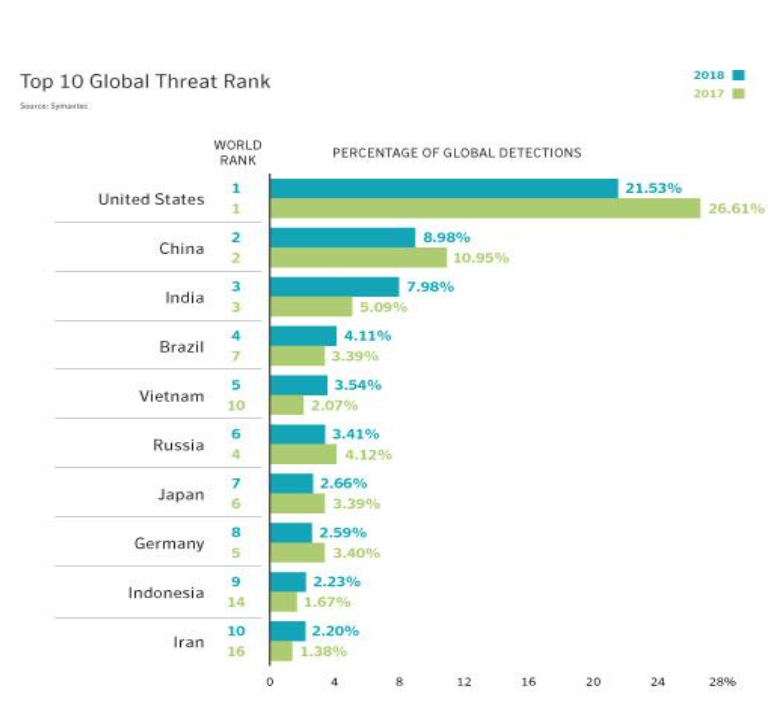
\includegraphics[width=.4\textwidth]{picture/Gambar 1.1.PNG}
\caption{Peringkat Ancaman Kejahatan Siber di Dunia}
\end{figure}

Namun pada tahun 2020 BSSN menyebutkan serangan siber di Indonesia meningkat hingga 6 kali lipat dari tahun 2019

\begin{center}
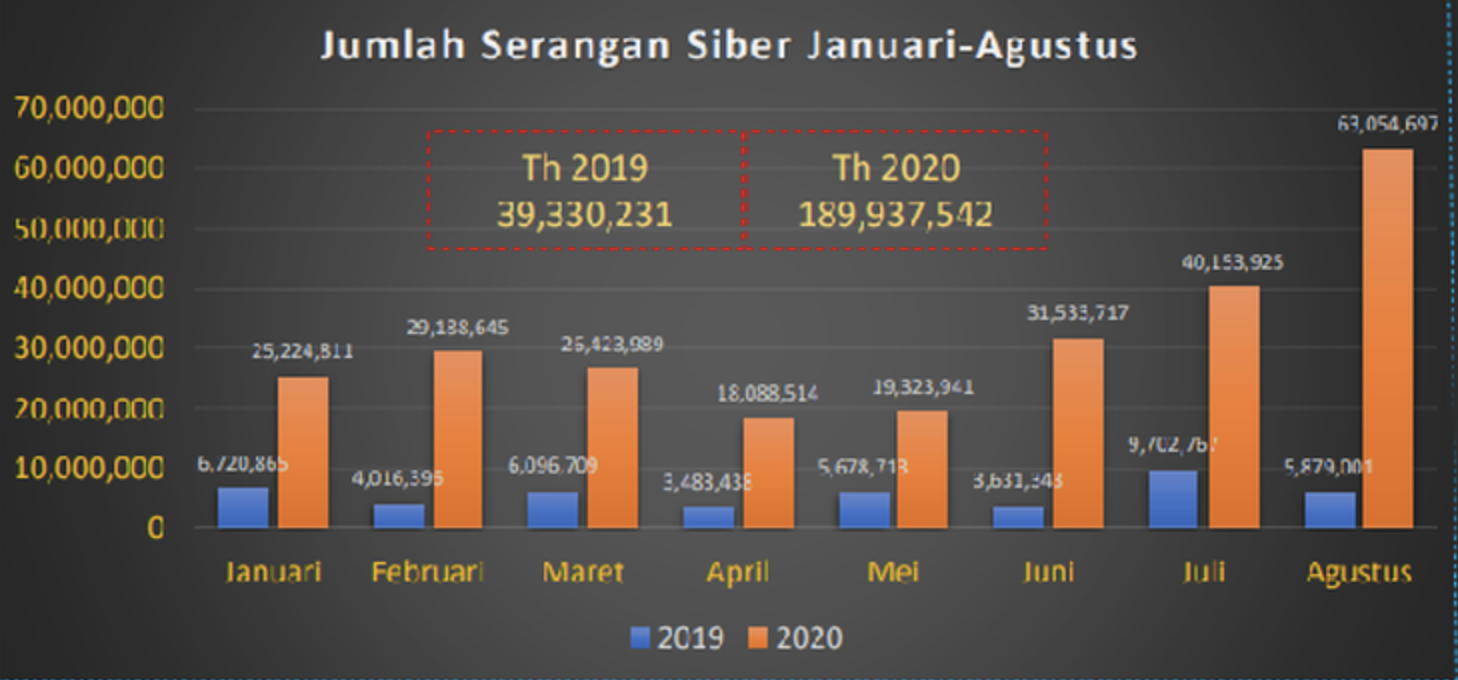
\includegraphics[width=.4\textwidth]{picture/Gambar 1.2.PNG}

\end{center}




%bagian dari Bab 2 penjelasan
\section{Related Work}
%bagian A. Keamanan Komputer
\subsection{Keamanan Komputer}
Arti dari keamanan komputer telah berubah dalam beberapa tahun terakhir. Sebelum masalah keamanan data/informasi menjadi populer, kebanyakan orang berpikir bahwa keamanan komputer difokuskan pada alat alat komputer secara fisik. Secara tradisional, fasilitas komputer secara fisik dilindungi karena tiga alasan:
\begin{itemize}
    \item Untuk mencegah pencurian atau kerusakan hardware
    \item Untuk mencegah pencurian atau kerusakan informasi
    \item Untuk mencegah gangguan layanan
\end{itemize}

Prosedur yang sangat ketat untuk akses ke ruang server diaplikasikan oleh sebagian besar organisasi, dan prosedur ini sering digunakan untuk mengukur level keamanan computer. Dengan adanya akses jarak jauh atau remote terminal, jaringan yang sudah banyak serta teknologi internet yang berkembang pesat maka perlindungan secara fisik sudah jarang atau tidak dapat lagi digunakan untuk mengukur level keamanan. Meskipun demikian, masih ada beberapa perusahaan yang masih melindungi fasilitas fisik server mereka dengan peralatan cangih tetapi kurang memperhatikan perlindungan terhadap data atau informasi itu sendiri yang disimpan dalam server. Walupun nilai data atau informasi tersebut beberapa kali lebih besar dari nilai hardware.

Oleh karena itu konsep atau definisi computer security atau keamanan computer saat ini manjadi lebih luas atau bisa juga didefinisikan sebagai berikut: keamanan komputer dirancang untuk melindungi komputer dan segala sesuatu yang berkaitan dengan itu, bangunannya, workstation dan printer, kabel, dan disk dan media penyimpanan lainnya. Yang paling penting, keamanan komputer melindungi informasi yang disimpan dalam sistem anda. Keamanan komputer tidak hanya dirancang untuk melindungi terhadap penyusup dari luar yang masuk ke sistem, tetapi juga bahaya yang timbul dari dalam seperti berbagi password dengan teman, gagal atau tidak dilakukan untuk backup data, menumpahkan kopi pada keyboard dan sebagainya.

Didalam information security sering juga dikenal CIA Triad atau segitiga confidentiality (kerahasiaan), integrity (integritas), dan availability (ketersediaan). Kerahasiaan, integritas dan ketersediaan, yang dikenal sebagai segitiga CIA ini adalah model yang dirancang untuk memandu kebijakan untuk keamanan informasi dalam sebuah organisasi. Model ini juga kadang-kadang disebut sebagai triad AIC (ketersediaan, integritas dan kerahasiaan) untuk menghindari kebingungan dengan Central Intelligence Agency. Unsur-unsur dari tiga serangkai tersebut dianggap tiga komponen yang paling penting dari system keamanan.

Bila bicara kerahasiaan sama dengan bicara privasi. Langkah-langkah yang dilakukan untuk menjamin kerahasiaan dirancang untuk mencegah informasi rahasia dan sensitif di ambil oleh orang yang tidak berhak. Oleh karena itu access harus dibatasi hanya untuk mereka yang berwenang saja yang dapat melihat data yang sensitive atau rahasia tersebut.

Sebuah sistem komputer yang aman harus menjaga agar informasi selalu tersedia untuk pengguna. Ketersediaan berarti bahwa perangkat keras dan perangkat lunak sistem komputer terus bekerja secara efisien dan bahwa sistem ini mampu pulih dengan cepat dan benar jika ada bencana.

Integritas melibatkan beberapa unsur yaitu: menjaga konsistensi, akurasi, dan kepercayaan dari data melalui seluruh siklus hidupnya. Data tidak boleh diubah pada saat ditransmisikan. Dalam hal ini harus diambil langkah langkah untuk memastikan bahwa data tidak dapat diubah oleh orang yang tidak berhak dan tidak kurang suatu apapun serta benar adanya.

Dalam keamanan komputer ada tiga komponen yang selalu menjadi diskusi:
\begin{itemize}
    \item Kerentanan: adalah kelemahan dari komputer yang memungkinkan penyerang untuk masuk ke sistem jaringann informasi.
    \item Ancaman: adalah kemungkinan bahaya yang mungkin mengeksploitasi kerentanan untuk melakukan gangguan pada system keamanan dan karena itu dapat menyebabkan kemungkinan bahaya bagi organisasi.
    \item Penanggulangan: adalah suatu tindakan, perangkat, prosedur, atau teknik yang mengurangi ancaman, kerentanan, atau serangan dengan menghilangkan atau mencegah, dengan meminimalkan kerugian itu dapat menyebabkan, atau dengan menemukan dan melaporkan masalah system keamanan sehingga tindakan korektif dapat diambil.
\end{itemize}

%bagian B Intrusion Detection System (IDS)
\subsection{Intrusion Detection System (IDS)}
merupakan sistem untuk mendeteksi adanya “intrusion” yang dilakukan oleh “intruder” atau “pengganggu atau penyusup” di jaringan. IDS (Intrusion Detection System) sangat mirip seperti alarm, yaitu IDS (Instrusion Detection System) akan memperingati bila terjadinya atau adanya penyusupan pada jaringan. IDS (Intrusion Detection System) dapat didefinisikan sebagai kegiatan yang bersifat anomaly, incorrect, inappropriate yang terjadi di jaringan atau host. IDS (Intrusion Detection System) adalah sistem keamanan yang bekerja bersama Firewall untuk mengatasi Intrusion.

\begin{center}
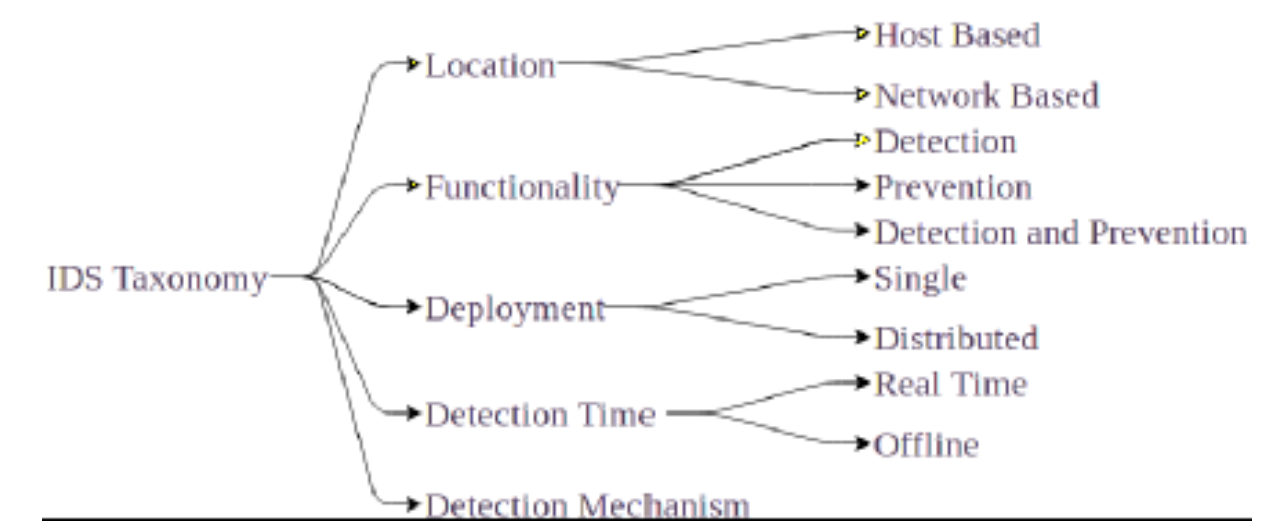
\includegraphics[width=.4\textwidth]{picture/Gambar 2.2.1.PNG}

\end{center}

Taksonomi pada IDS dibagi menjadi lima bagian. Setiap bagian tersebut haru diperhitungkan berdasarkan tujua penggunaannya dan keuntungan kerugianny Kelima hal tersebut adalah lokasi, fungs penyebarannya, waktu pendeteksiannya da mekanisme pendeteksiannya (Pharate, dkk., 2015). Gambar 2.2.1 menjelaskan tentang taksonomi dari IDS.

\begin{center}
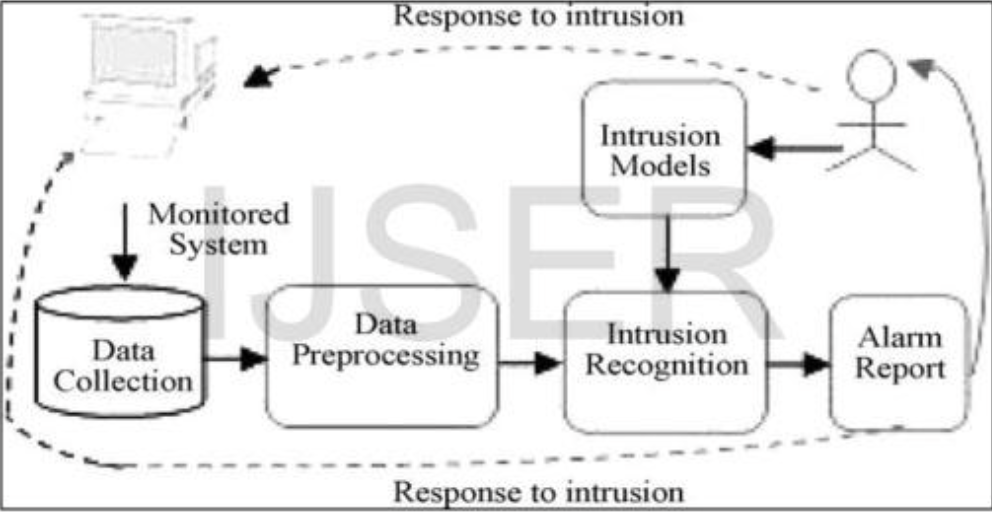
\includegraphics[width=.4\textwidth]{picture/Gambar 2.2.2.PNG}
\end{center}

Untuk membangun IDS setidaknya diperlukan 5 (lima) tahapan yaitu Data Collection, Data Preprocessing, Intrusion Recognition, Reporting dan Respone. IDS () juga memiliki cara kerja dalam menganalisa apakah paket data yang dianggap sebagai intrusion oleh intruser. Cara kerja IDS () dibagi menjadi dua, yaitu :

\subsubsection{Knowledge Based (Misuse Detection)}
Knowledge Based pada IDS (Intrusion Detection System) adalah cara kerja IDS (Intrusion Detection System) dengan mengenali adanya penyusupan dengan cara menyadap paket data kemudian membandingkannya dengan database rule pada IDS (Intrusion Detection System) tersebut. Database rule tersebut dapat berisi signature – signature paket serangan. Jika pattern atau pola paket data tersebut terdapat kesamaan dengan rule pada database rule pada IDS (Intrusion Detection System), maka paket data tersebut dianggap sebagai seranganm dan demikian juga sebaliknya, jika paket data tersebut tidak memiliki kesamaan dengan rule pada database rule pada IDS(Intrusion Detection System), maka paket data tersebut tidak akan dianggap serangan.

\subsubsection{Behavior Based (Anomaly Based)}
Behavior Base adalah cara kerja IDS (Intrusion Detection System) dengan mendeteksi adanya penyusupan dengan mengamati adanya kejanggalan– kejanggalan pada sistem, aatu adanya keanehan dan kejanggalan dari kondiri pada saat sistem normal, sebagai: adanya penggunaan memory yang melonjak secara terus menerus atau terdapatnya koneksi secara paralel dari satu IP dalam jumlah banyak dan dalam waktu yang bersamaan. Kondisi tersebut dianggap kejanggalan yang selanjutnya oleh IDS (Intrusion Detection System) Anomaly Based ini dianggap sebagai serangan. Intrusion itu sendiri didefinisikan sebagai kegiatan yang bersifat anomaly, incorrect, inappropite yang terjadi di jaringan atau di host tersebut. Intrusion tersebut kemudian akan diubah menjadi “rules” ke dalam IDS (Intrusion Detection System). Sebagai contoh, intrusion atau gangguan seperti port scanning yang dilakukan oleh intruder. Oleh karena itu IDS (Intrusion Detection System) ditujukan untuk meminimalkan kerugian yang dapat ditimbulkan dari intrusion. Kelebihan yang akan di dapatkan dengan menggunakan IDS (Intrusion Detection System) sebagai metode Keamanan:
\begin{itemize}
    \item Memiliki Akurasi keamanan yang baik. IDS (Intrusion Detection System) haruslah memiliki akurasi atau ketelitian, jadi IDS (Intrusion Detection System) yang baik adalah IDS (Intrusion Detection System) yang memiliki ketelitian yang baik untuk mengenal intrusion atau gangguan. Pada saat sekrarang ini IDS (Intrusion Detection System) telah memiliki ketelitian tinggi, yaitu mampu secara realtime mendeteksi dan melakukan blocking terhadap tindakan yang mencurigakan. Selain itu IDS () juga harus mampu memeriksa dan menganalisa pattern objek secara menyeluruh seperti paket – paket data baik Header Paket maupun Payload yang dipergunakan serta membedakan paket data yang keluar masuk dalam lalu lintas jaringan sehingga dapat mengenal benar karateristik trafic.
    \item Mampu Mendeteksi dan Mencegah Serangan. IDS (Intrusion Detection System) haruslah dapat mendeteksi serangan dn juga mampu untuk melakukan pencegahan terhadap serangan tersebut, IDS (Intrusion Detection System) yang baik dalam mengatasi serangan adalah IDS (Intrusion Detection System).
    \item Memiliki cakupan yang Luas dalam Mengenal Proses Attacking. IDS (Intrusion Detection System) haruslah memiliki pengetahuan yang luas, dapat mengenal serangan apa yang belum dikenalnya, seperti contoh IDS(Intrusion Detection System) harus mampu mendeteksi serangan DOS mempergunakan analisis signature dan mampu mendeteksi segala sesuatu yang mencurigakan. IDS (Intrusion Detection System) yang baik dalam pengenalan attacking adalah IDS (Intrusion Detection System).
    \item Dapat memeberikan Informasi tentang ancaman – ancaman yang terjadi.
    \item Memiliki tingkat Forensik yang canggih dan mampu menghasilkan reporing yang baik. Memiliki sensor yang dapat dipercaya untuk memastikan pendeteksian dan pencegahan.
\end{itemize}

\subsection{Data Mining}
Data mining adalah teknologi yang mengombinasikan metode analisis tradisional dan algoritma yang canggih agar
proses data besar lebih cepat diproses. Data mining biasa disebut dengan sebutan yang sering digunakan untuk mencari pengetahuan yang tersembunyi didalam database. Data mining menggunakan teknik statistika, matematika, kecerdasan buatan, dan machine learining untuk mengekstraksi dan menganalisa informasi yang terdapat dalam database besar. (Turban et al, 2005).

Analisis yang dilakukan data mining lebih maksimum dibandingkan sistem pendukung keputusan tradisional yang banyak digunakan. Data mining mengatasi masalah-masalah bisnis dengan cara tradisional yang menggunakan banyak waktu da biaya yang tinggi. Data mining menjelajahi basis data untuk mengetahui pola yang tersembunyi, serta mencari informasi agar dapat memprediksi yang bisa saj dilupakan oleh pembisnis karena kemungkinan besar mereka tidak menduganya.

Pada perkembangan teknologi saat ini, proses pengumpulan data serta penyimpanannya telah mudah dijalankan walaupun data tersebut berukuran besa sehingga data mining melakukan proses pencarian secara mudah dan otomatis mencari informasi yang berguna dalam penyimpanan data yang mempunyai ukura yang besar. Istilah ini biasa disebut dengan Knowledge Discovery in Database (KDD) yang digunakan secara bergantian untuk memberikan penjelasan tentang prose pencarian informasi yang tersembunyi dalam suatu basis data yang besar. Sebenarnya konsep ini berkaitan satu sama lain walaupun konsepnya berbeda.

\subsection{Mechine Learning}
\begin{itemize}
    \item Machine Learning dapat digunakan untuk melakukan penggalian informasi pada data set yang tersedia. Dengan menggunakan perhitungan statistika dan algoritma yang matematis, machine learning dapat mengetahui informasi yang tersembunyi, pola dan hubungan antar atribut dalam sebuah data set. Fungsi ini menjadi sangat berguna untuk mengetahui data yang mencurigakan.
    \item Machine Learning juga dapat digunakan untuk mendeteksi serangan pada jaringan (J. dan Muthukumar, 2015). Pengembangan terhadap penggunaan machine learning telah dikembangkan untuk mengetahui algoritma yang terbaik untuk detect ion engine pada IDS Tabel 1 menunjukkan perbandingan performa antar algoritma yang diimplementasikan pada IDS .
\end{itemize}

\begin{center}
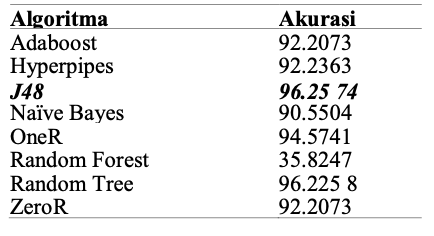
\includegraphics[width=.4\textwidth]{picture/Gambar 2.4.1.PNG}
\end{center}

\section{Metodologi}
\subsection{Random Forest}
Random Forest merupakan salah satu metode yang digunakan untuk menyelesaikan permasalahan. Metode ini merupakan metode pohon gabungan yang berasal dari metode classification and regression tree (CART) dan didasarkan pada teknik pohon keputusan (decision tree), sehingga mampu mengatasi masalah non-linier. Dalam random forest, banyak pohon ditumbuhkan, sehingga terbentuk suatu hutan (forest). Analisis selanjutnya akan dilakukan pada kelompok hutan tersebut.

Pada gugus data yang terdiri atas n amatan dan p peubah penjelas, prosedur melaksanakan random forest menurut Breiman (2001) dilakukan dalam tiga tahap. Tahap pertama atau tahap bootstrap, dilakukan penarikan contoh acak berukuran n dengan pemilihan pada gugus data. Berikutnya dengan menggunakan contoh bootstrap, pohon dibangun sampai mencapai ukuran maksimum (tanpa pemangkasan). Pembangunan pohon dilakukan dengan menerapkan random feature selection pada setiap proses pemilihan pemilah, yaitu m peubah penjelas dipilih secara acak dengan m < p, lalu pemilah terbaik dipilih berdasarkan m peubah penjelas tersebut. Terakhir, ulangi langkah satu dan dua sebanyak k kali, sehingga terbentuk sebuah hutan yang terdiri atas k pohon.

Random forest memprediksi respons suatu amatan dengan cara menggabungkan (aggregating) hasil prediksi k pohon. Untuk masalah klasifikasi, pohon yang dibangun adalah pohon klasifikasi sedangkan hasil prediksi random forest dipilih berdasarkan suara terbanyak, yaitu kategori atau kelas yang paling sering muncul sebagai hasil prediksi dari k pohon klasifikasi.

Untuk melakukan random forest yang menghasilkan variable importance, disarankan untuk menggunakan banyak pohon, misalnya seribu pohon atau lebih. Jika peubah penjelas yang dianalisis sangat banyak, nilai tersebut sebaiknya lebih besar agar variable importance yang dihasilkan semakin stabil (Breiman dan Cutler).

Serta berikut ini adalah kelebihan dan kekurangan pada Algoritma Random Forest. Kelebihannya yaitu dapat mengatasi noise dan missing value serta dapat mengatasi data dalam jumlah yang besar. Dan kekurangan pada algoritma Random Forest yaitu interpretasi yang sulit dan membutuhkan tuning model yang tepat untuk data.


\subsection{K-Nearest Neighbor}
Algoritma K-Nearest Neighbor (K-NN) adalah sebuah metode klasifikasi terhadap sekumpulan data berdasarkan pembelajaran  data yang sudah terklasifikasikan sebelumya. Termasuk dalam supervised learning, dimana hasil query instance yang baru diklasifikasikan berdasarkan mayoritas kedekatan jarak dari kategori yang ada dalam K-NN.

 Tahapan Langkah Algoritma K-NN
\begin{itemize}
    \item Menentukan parameter k (jumlah tetangga paling dekat).
    \item Menghitung kuadrat jarak eucliden objek terhadap data training yang diberikan.
    \item Mengurutkan hasil no 2 secara ascending (berurutan dari nilai tinggi ke rendah)
    \item Mengumpulkan kategori Y (Klasifikasi nearest neighbor berdasarkan nilai k)
    \item Dengan menggunakan kategori nearest neighbor yang paling mayoritas maka dapat dipredisikan kategori objek.
\end{itemize}

\subsection{Structural Risk Minimization (SVM)}
SVM digunakan untuk mencari hyperplane terbaik dengan memaksimalkan jarak antar kelas. Hyperplane adalah sebuah fungsi yang dapat digunakan untuk pemisah antar kelas. Dalam 2-D fungsi yang digunakan untuk klasifikasi antar kelas disebut sebagai line whereas, fungsi yang digunakan untuk klasifikasi antas kelas dalam 3-D disebut plane similarly, sedangan fungsi yang digunakan untuk klasifikasi di dalam ruang kelas dimensi yang lebih tinggi di sebut hyperplane.

\begin{center}
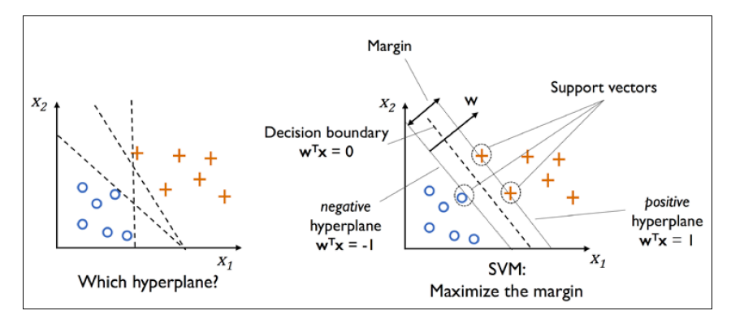
\includegraphics[width=.4\textwidth]{picture/Gambar 3.3.1.png}
\end{center}

Hyperplane yang ditemukan SVM diilustrasikan seperti Gambar 1 posisinya berada ditengah-tengah antara dua kelas, artinya jarak antara hyperplane dengan objek-objek data berbeda dengan kelas yang berdekatan (terluar) yang diberi tanda bulat kosong dan positif. Dalam SVM objek data terluar yang paling dekat dengan hyperplane disebut support vector. Objek yang disebut support vector paling sulit diklasifikasikan dikarenakan posisi yang hampir tumpang tindih (overlap) dengan kelas lain. Mengingat sifatnya yang kritis, hanya support vector inilah yang diperhitungkan untuk menemukan hyperplane yang paling optimal oleh SVM.

\subsection{Ensemble Learning}
Kenyataan bahwa pendekatan ensemble learning mampu memberikan solusi prediksi yang lebih akurat daripada model-model tunggal dapat ditemui dari berbagai paper di jurnal ilmiah.  Teknik-teknik ensemble yang mengandalkan variasi dari pendekatan random forest dan boosting mampu memberikan prediksi dengan akurasi yang sangat baik.  Random forest bekerja dengan membuat model-model penyusun ensemble sedemikian rupa sehingga berbagai kemungkinan dapat terakomodir secara maksimal, sedangkan boosting bekerja secara iteratif sehingga kasus-kasus yang tidak mudah diprediksi menjadi bukan masalah lagi.

Kemampuan pendekatan ensemble ini tidak hanya tertuang pada berbagai paper ilmiah, namun juga dapat dilihat pada penyelesaian kasus-kasus aplikatif seperti yang dapat dilihat pada kompetisi data science Kaggle ompetisi ini terbuka bagi pegiat data science dan data mining untuk memberikan solusi prediktif dari kasus-kasus yang disampaikan oleh banyak perusahaan besar berskala internasional.  Setiap tim atau individu dipersilakan mengembangkan solusi dan menyajikan prediksinya untuk kemudian dinilai.  Mereka yang memberikan prediksi dengan akurasi yang paling tinggi yang dinyatakan sebagai pemenang.  Peringkat tiga besar dalam lima tahun terakhir dari kompetisi ini didominasi oleh mereka yang menggunakan pendekatan ensemble yang digabungkan dengan berbagai macam algoritma dasar.

Berdasarkan apa yang berkembang saat ini, pendekatan ensemble dalam pemodelan prediktif menjadi pilihan tepat bagi mereka yang berupaya memperoleh prediksi yang memuaskan dengan cara yang sangat mudah untuk dikerjakan.  Hal senada juga telah dikemukanan oleh Mu Zhu (University of Waterloo) pada jurnal The American Statistician pada tahun 2008.

\section{Result and Discussion}
\subsection{Result}
Random Forest merupakan salah satu metode yang digunakan untuk

\subsection{Performa}
Random Forest merupakan salah satu metode yang digunakan untuk

\subsection{Random Forest}
Random Forest merupakan salah satu metode yang digunakan untuk


\section{Kesimpulan}
Pada saat keamanan komputer sangat penting. salah satu cara meningkatkan keamanan komputer adalah kita menggunakan IDS. Ada beberapa algoritma yang dapat digunakan, masing-masing algoritama memiliki kelebihan dan kekurangan.
Dengan tersebut keamanan komputer akan terus terjaga.

\bibliographystyle{IEEEtran}
\bibliography{bibliography.bib}


\end{document}
